%!TEX root = ../paper.tex

\begin{figure}
	\centering
	\beforeFinalVersion{Remove ticks and labels.}
	%!TEX root = ../paper.tex

% Ferdosi Set 2
\begin{subfigure}{0.23\textwidth}
	\centering
	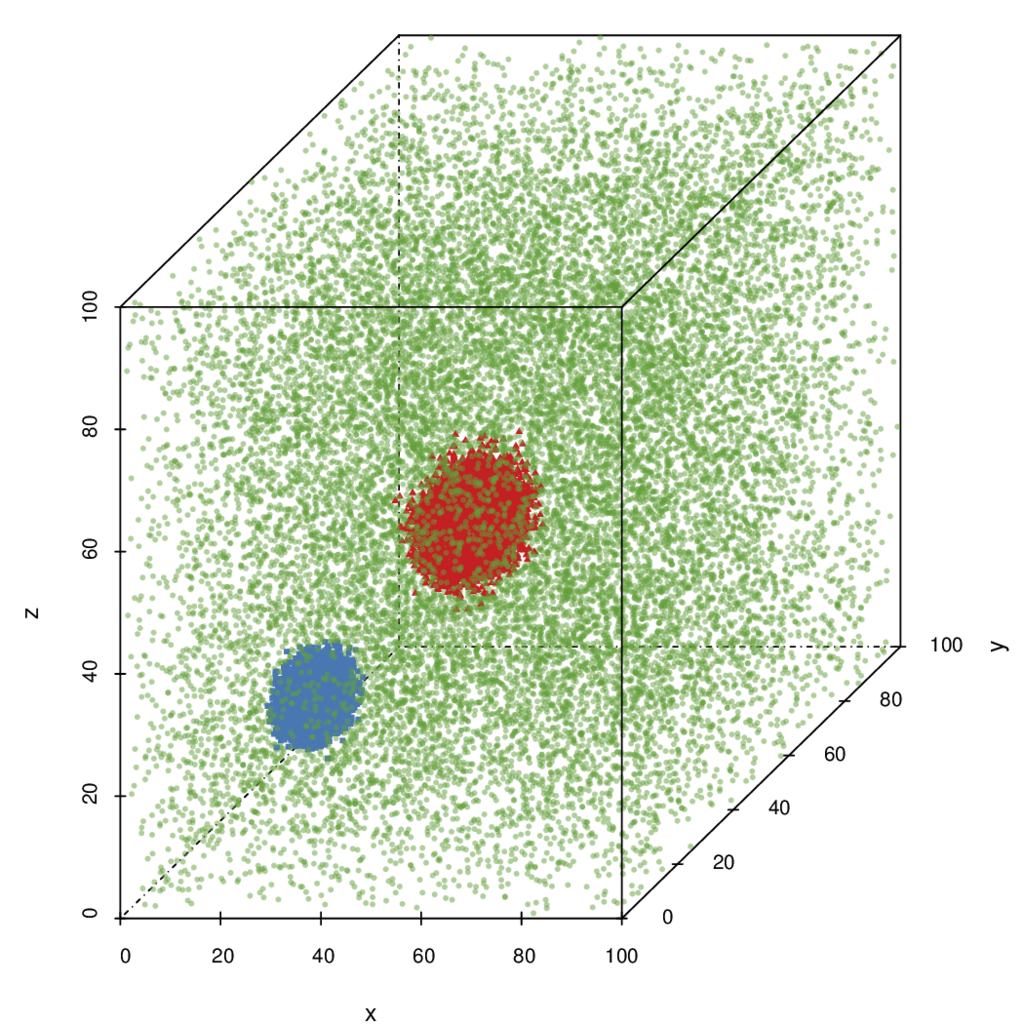
\includegraphics[width=\textwidth]{experiment/img/datasetplot_ferdosi_2_60000}
	\caption{Set \ferdosiTwo}
	\label{fig:experiment:multisphere:ferdosi2}
\end{subfigure}	
% Ferdosi Set 3
\begin{subfigure}{0.23\textwidth}
	\centering
	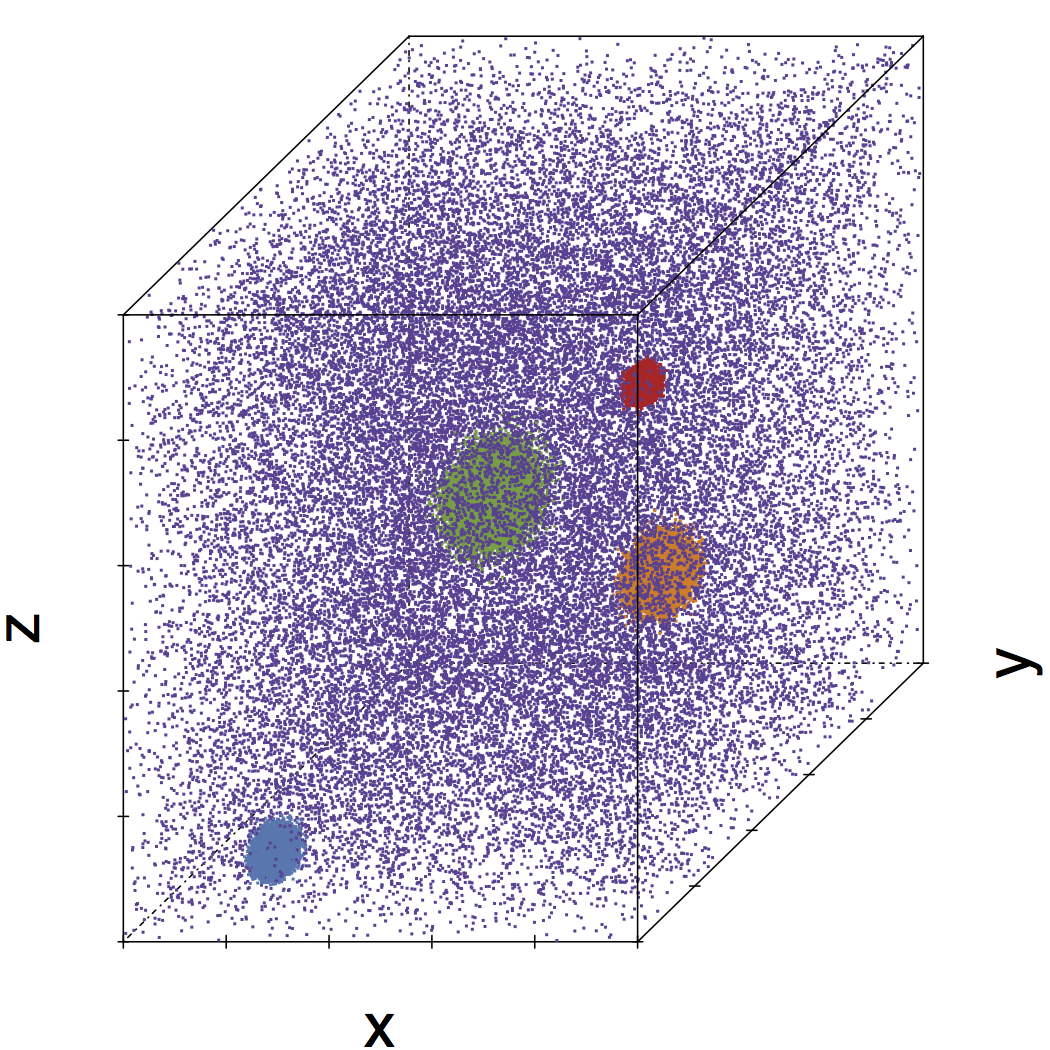
\includegraphics[width=\textwidth]{experiment/img/datasetplot_ferdosi_3_120000}
	\caption{Set \ferdosiThree}
	\label{fig:experiment:multisphere:ferdosi3}
\end{subfigure}	
% Baakman 2
\begin{subfigure}{0.23\textwidth}
	\centering
	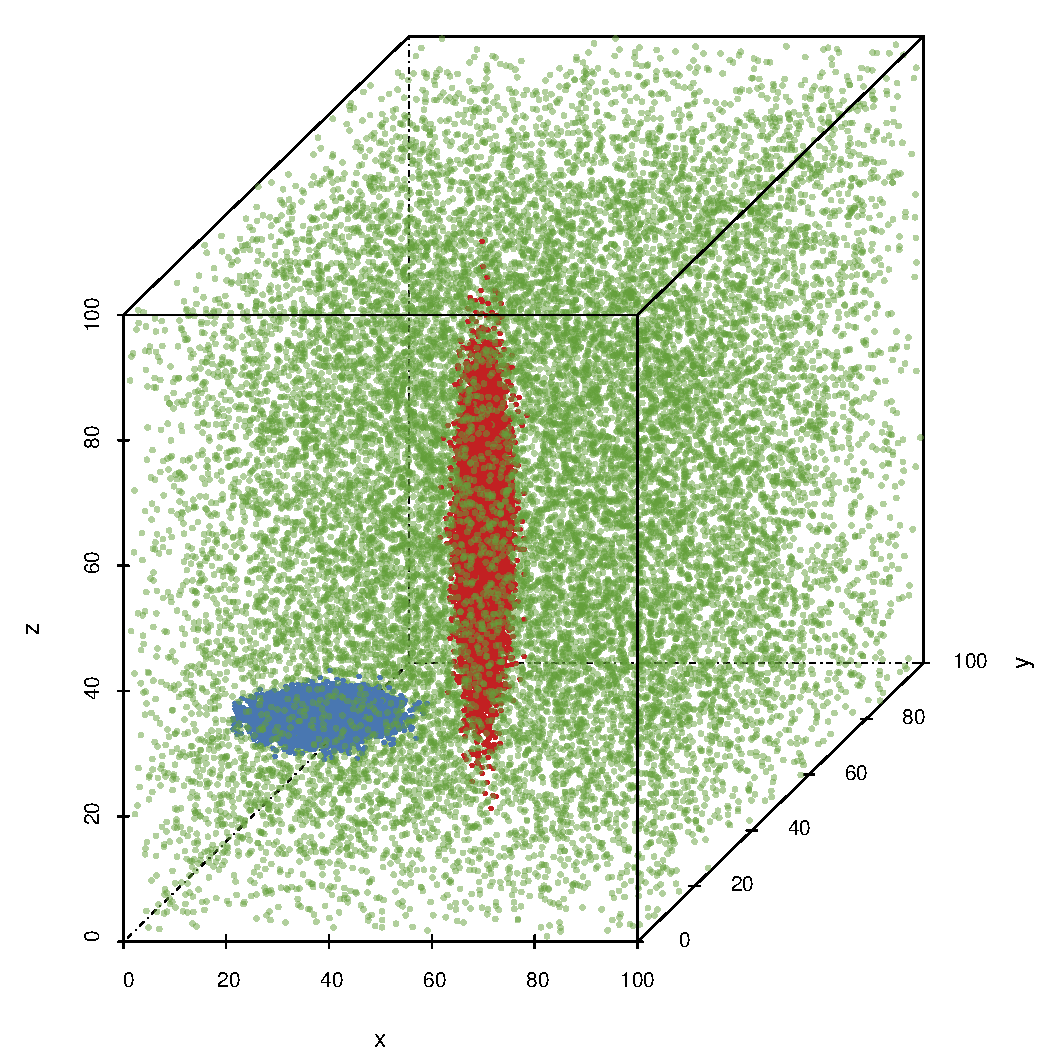
\includegraphics[width=\textwidth]{experiment/img/datasetplot_baakman_2_60000}
	\caption{Set \baakmanTwo}
	\label{fig:experiment:multisphere:baakman2}
\end{subfigure}			
% Baakman 3
\begin{subfigure}{0.23\textwidth}
	\centering
	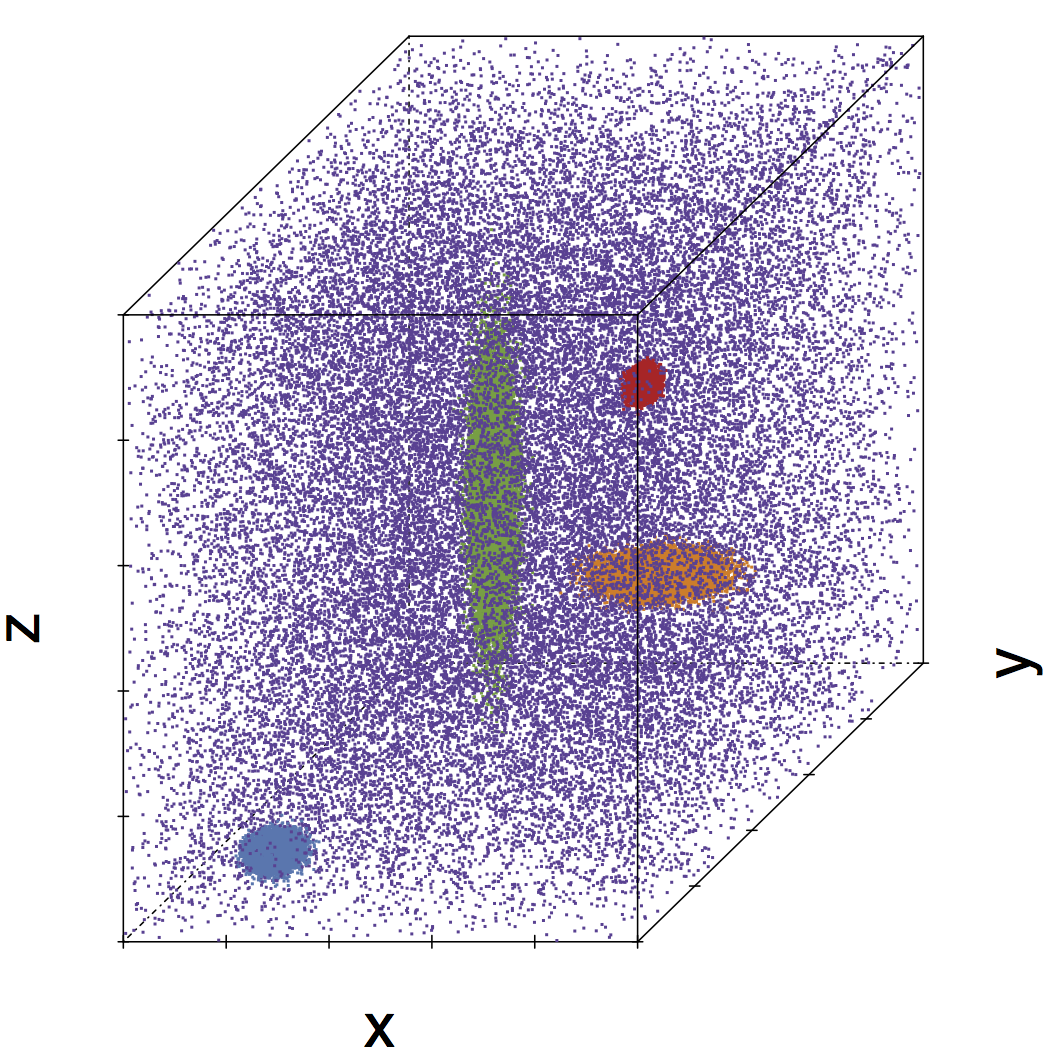
\includegraphics[width=\textwidth]{experiment/img/datasetplot_baakman_3_120000}
	\caption{Set \baakmanThree}
	\label{fig:experiment:multisphere:baakman3}
\end{subfigure}
	\caption{Scatter plot representation of the datasets defined in \cref{tab:experiment:multisphere:sets}, the colors used for the different components correspond with the colors used in that table.}
	\label{fig:experiment:multisphere:sets}
\end{figure}

\begin{table*}
	\centering
	%!TEX root = ../paper.tex

\begin{tabular}{@{}cclS[table-format=+1.1e+1,scientific-notation=true,round-mode=places,round-precision=1]l@{}}
\toprule
Set 			&~						& Component					& {Number} 	& Distribution\\
\midrule
% Ferdosi 2
\ferdosiTwo 	&\legendComponentOne	& Trivariate Gaussian 1		& 20000		& $\gaussDist{[25, 25, 25]}{\diag(5)}$\\
~ 				&\legendComponentTwo	& Trivariate Gaussian 2		& 20000		& $\gaussDist{[45, 45, 45]}{\diag(11)}$\\
~ 				&\legendComponentNoise	& Uniform random background	& 20000		& $\uniformDist{[0, 0, 0]}{[100, 100, 100]}$\\
% Baakman 2
\hline
\baakmanTwo		&\legendComponentOne	& Trivariate Gaussian 1		& 20000		& $\gaussDist{[25, 25, 25]}{\diag([5^2, \sqrt{5}, \sqrt{5}])}$\\
~ 				&\legendComponentTwo	& Trivariate Gaussian 2		& 20000		& $\gaussDist{[45, 45, 45]}{\diag([\sqrt{11}, \sqrt{11}, 11^2])}$\\
~ 				&\legendComponentNoise	& Uniform random background	& 20000		& $\uniformDist{[0, 0, 0]}{[100, 100, 100]}$\\
% Ferdosi 3
\hline
\ferdosiThree	&\legendComponentOne 	& Trivariate Gaussian 1 	& 20000		& $\gaussDist{[24, 10, 10]}{\diag(2)}$\\
~ 				&\legendComponentTwo	& Trivariate Gaussian 2 	& 20000		& $\gaussDist{[33, 70, 40]}{\diag(10)}$\\
~ 				&\legendComponentThree	& Trivariate Gaussian 3 	& 20000		& $\gaussDist{[90, 20, 80]}{\diag(1)}$\\
~ 				&\legendComponentFour	& Trivariate Gaussian 4 	& 20000		& $\gaussDist{[60, 80, 23]}{\diag(5)}$\\
~ 				&\legendComponentNoise	& Uniform random background	& 40000		& $\uniformDist{[0, 0, 0]}{[100, 100, 100]}$\\
% Baakman 3
\hline
\baakmanThree	&\legendComponentOne 	& Trivariate Gaussian 1 	& 20000		& $\gaussDist{[24, 10, 10]}{\diag([4, \sqrt{2}, \sqrt{2}])}$\\
~ 				&\legendComponentTwo	& Trivariate Gaussian 2 	& 20000		& $\gaussDist{[33, 70, 40]}{\diag([\sqrt{10}, \sqrt{10}, 100])}$\\
~ 				&\legendComponentThree	& Trivariate Gaussian 3 	& 20000		& $\gaussDist{[90, 20, 80]}{\diag(1)}$\\
~ 				&\legendComponentFour	& Trivariate Gaussian 4 	& 20000		& $\gaussDist{[60, 80, 23]}{\diag([25, \sqrt{5}, \sqrt{5}])}$\\
~ 				&\legendComponentNoise	& Uniform random background	& 40000		& $\uniformDist{[0, 0, 0]}{[100, 100, 100]}$\\
\bottomrule
\end{tabular}
	\caption{The datasets with multiple Gaussian distributions embedded in uniform noise. This table has the same structure as \cref{tab:experiment:singlesphere:sets}.} 	
	\label{tab:experiment:multisphere:sets}
\end{table*}

%General
\Cref{tab:experiment:multisphere:sets} defines the datasets that consist of uniform random noise and multiple Gaussian distributions, a scatter plot representation of the sets is shown in \cref{fig:experiment:multisphere:sets}. 
	% Ferdosi 2
	Dataset \ferdosiTwo consists of two Gaussian distributions embedded in noise, the first Gaussian component is significantly denser than the second. The spheres are placed in such a way that they are unlikely to overlap. 
	% Baakman 2
	The procedure outlined in \cref{s:experiment:singlesphere} for the creation of dataset \baakmanOne was used to derive dataset \baakmanTwo from set \ferdosiTwo.
	% Ferdosi Three
	Dataset \ferdosiThree embeds four Gaussians, with eigenspheres with notably differencing radii in the uniform random back ground. It is unlikely that these distributions overlap due to their placement. 
	%Baakman 3
	The last dataset, \baakmanThree, is a variation on \ferdosiThree, created with method that was used for the definition of dataset \baakmanTwo from \baakmanOne. 

%Hypothesis
	% Ferdosi 2
	\todo[inline]{Expectation ferdosi 2}
	% Baakman 2
	\todo[inline]{Expectation baakman 2}
	% Ferdosi 3
	\todo[inline]{Expectation ferdosi 3}
	% Baakman 3
	\todo[inline]{Expectation baakman 3}	